\begin{figure}
 \caption{Network Topology Diagram}
  \centering
   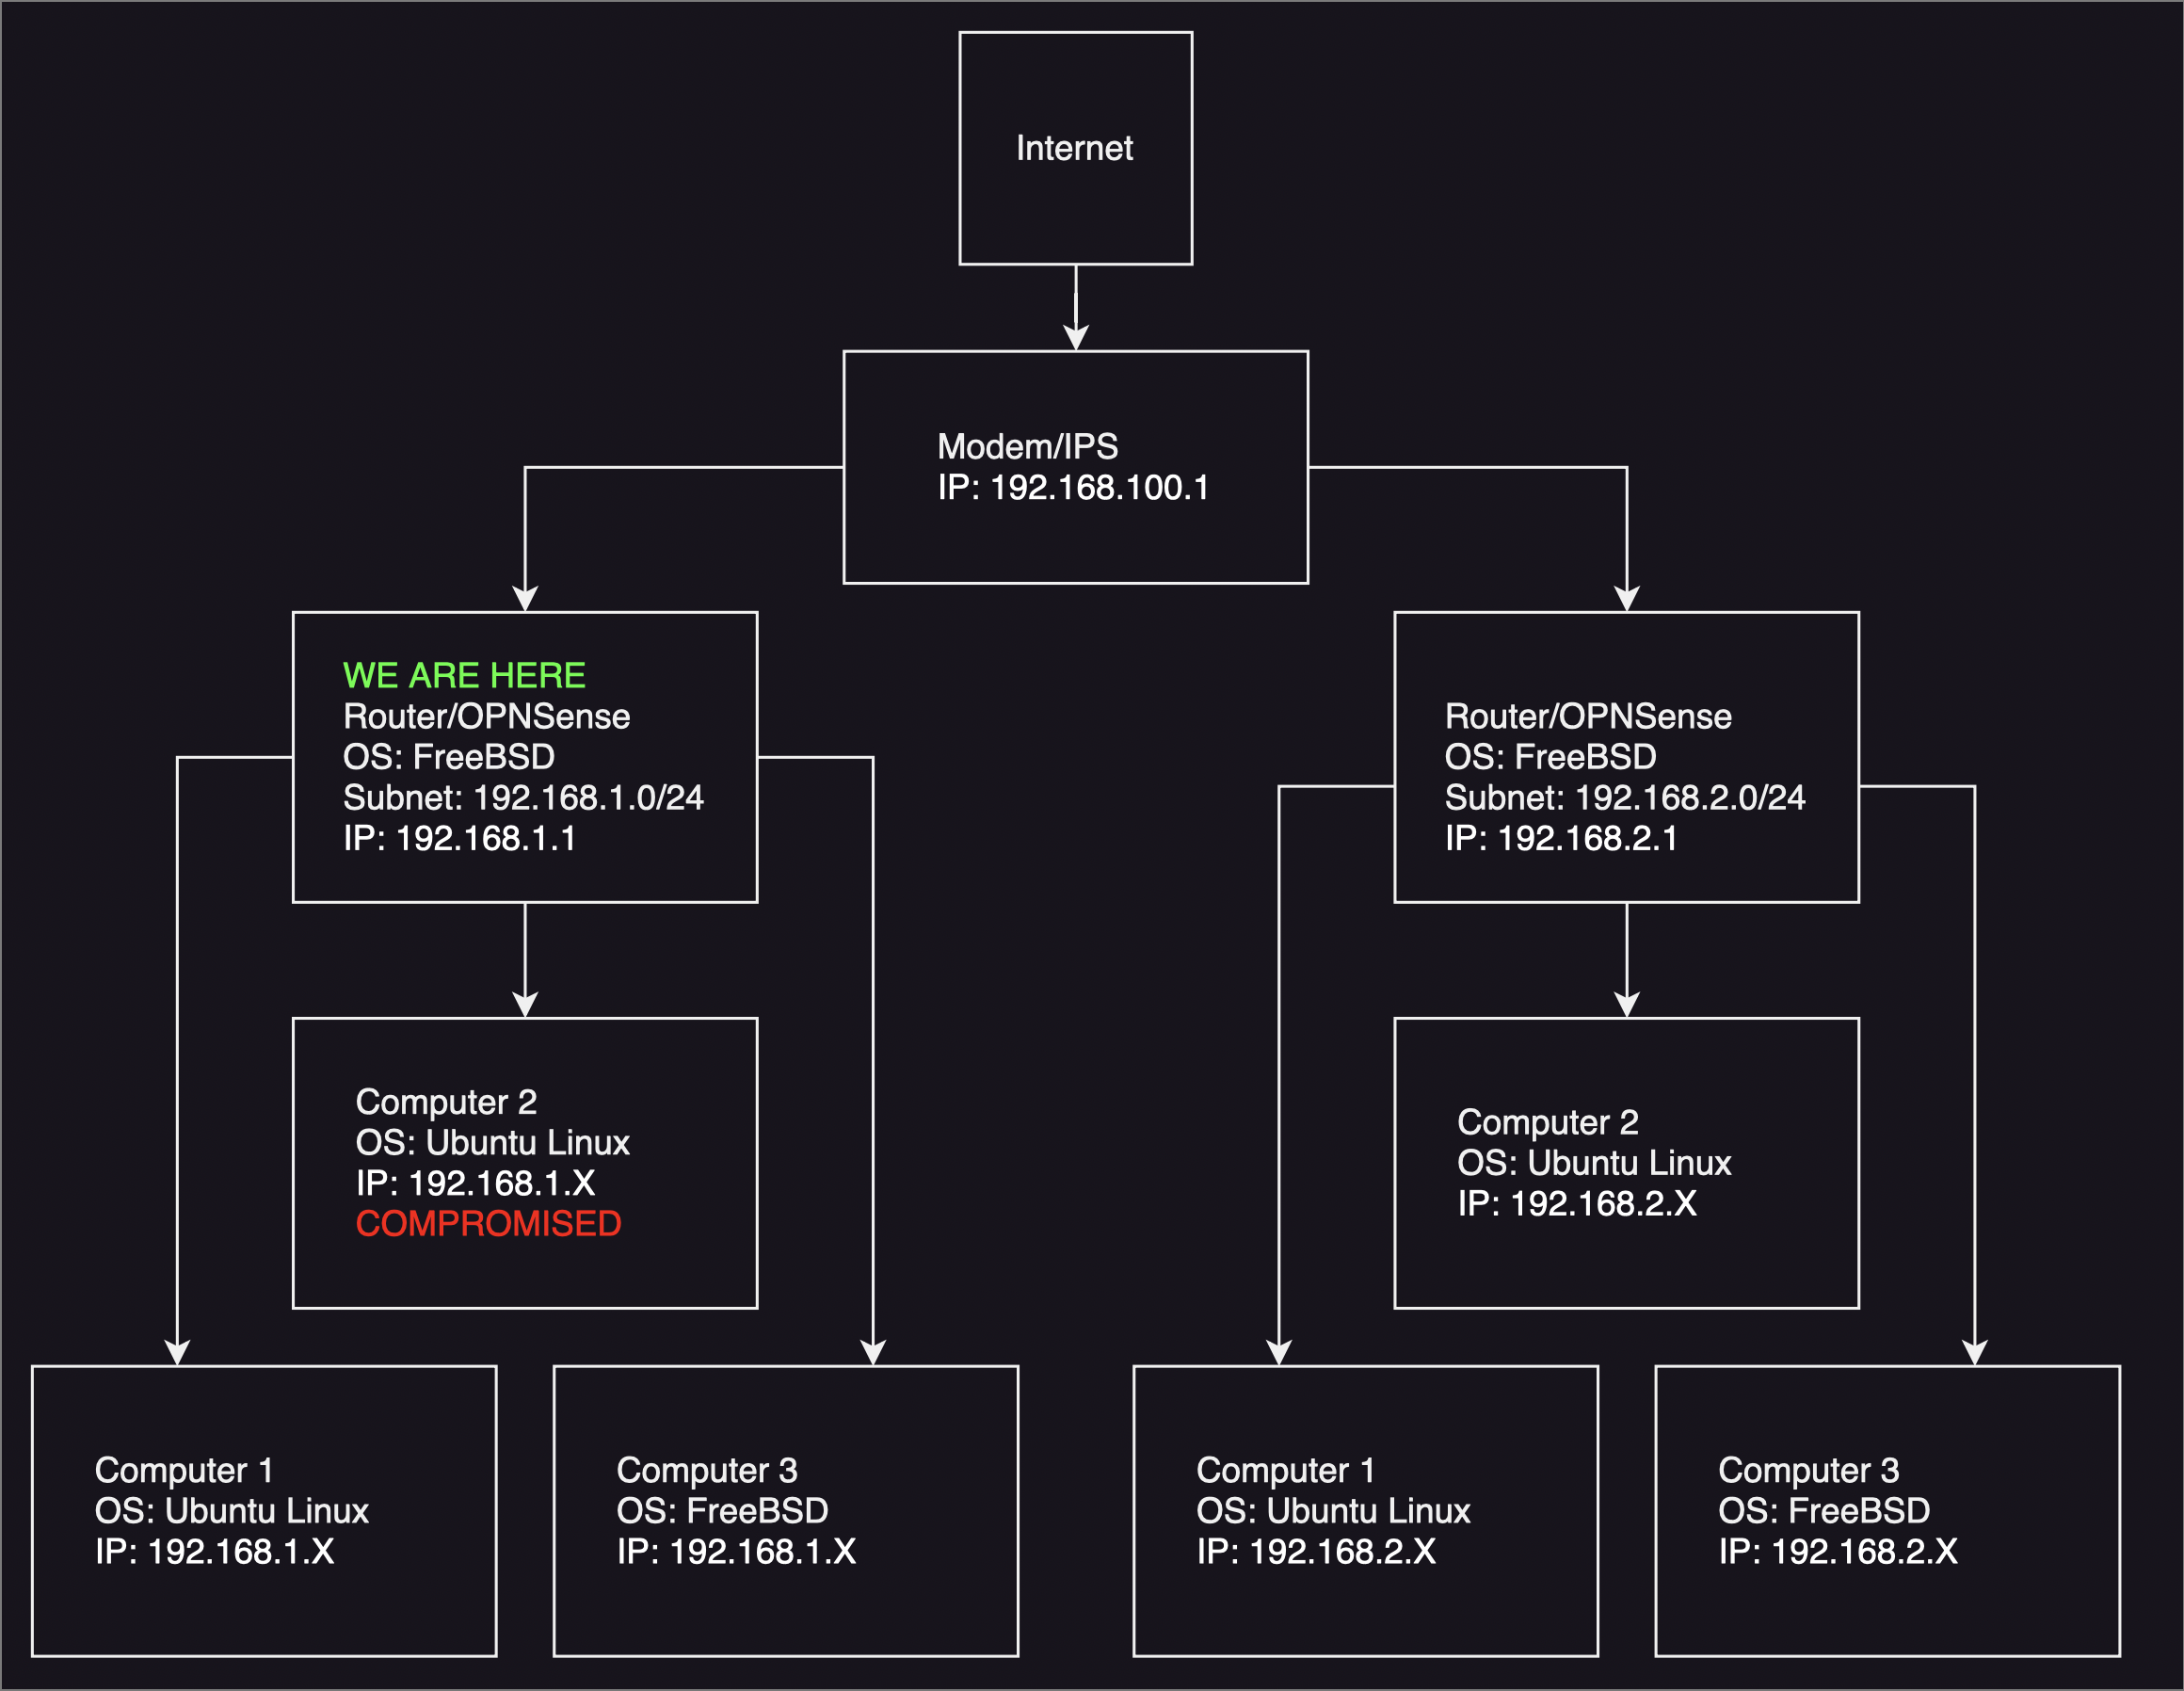
\includegraphics[width=0.5\textwidth]{diagram.png}
   \label{fig:network-topology}
\end{figure}

%-------------------------------------------------------------------------------

Our threat model involves a scenario where an adversary has successfully compromised a company device within a subnet on the company network. Figure~\ref{fig:network-topology} depicts the network topology in which this threat model takes place: three interconnected computers form a subnet, with one of these computers already compromised. In this scenario, the attacker is assumed to possess the following capabilities:
\begin{itemize}
    \item \textbf{Basic User Access:} The attacker has basic user privileges on the compromised system.
    \item \textbf{Network Reconnaissance:} The attacker can perform network reconnaissance by scanning the network.
    \item \textbf{System Persistence:} The attacker can maintain persistent access to the compromised device.
\end{itemize}
Given these capabilities, the attacker seeks to gain valuable reconnaissance information, identify other devices on the network, and exploit any discovered vulnerabilities that could facilitate lateral movement. The \texttt{ip-shuffle} script aims to counter these activities by dynamically assigning random IP addresses to network interfaces, making it difficult for the attacker to establish a static view of the network and impeding their ability to conduct effective reconnaissance.
